%!TEX program=xelatex

\documentclass[11pt]{ctexart}  
\usepackage[top=2cm, bottom=2cm, left=2cm, right=2cm]{geometry}  
\usepackage{algorithm}  
\usepackage{algorithmicx}  
\usepackage{algpseudocode}  
\usepackage{amsmath}  
\usepackage{graphicx}
\usepackage{amsmath}
\usepackage{amssymb}
\usepackage{enumerate}
\usepackage{booktabs}
\usepackage{fontspec}
\usepackage{listings}
\usepackage{xcolor}

\newfontfamily\monaco{Monaco}
\definecolor{mygreen}{rgb}{0,0.6,0}
\definecolor{mygray}{rgb}{0.5,0.5,0.5}
\definecolor{mymauve}{rgb}{0.58,0,0.82}
\lstset{ %
backgroundcolor=\color{white},      % choose the background color
basicstyle=\footnotesize\ttfamily,  % size of fonts used for the code
columns=fullflexible,
tabsize=4,
breaklines=true,               % automatic line breaking only at whitespace
captionpos=b,                  % sets the caption-position to bottom
commentstyle=\color{mygreen},  % comment style
escapeinside=``,        % if you want to add LaTeX within your code
keywordstyle=\color{blue},     % keyword style
stringstyle=\color{mymauve}\ttfamily,  % string literal style
frame=single,
rulesepcolor=\color{red!20!green!20!blue!20},
language=python,
}

\floatname{algorithm}{算法}
\renewcommand{\algorithmicrequire}{\textbf{输入:}}  
\renewcommand{\algorithmicensure}{\textbf{输出:}} 

\title{密码学实验报告9}
\author{张天辰 17377321}

\makeatletter
\newenvironment{breakablealgorithm}
  {% \begin{breakablealgorithm}
   \begin{center}
     \refstepcounter{algorithm}% New algorithm
     \hrule height.8pt depth0pt \kern2pt% \@fs@pre for \@fs@ruled
     \renewcommand{\caption}[2][\relax]{% Make a new \caption
       {\raggedright\textbf{\ALG@name~\thealgorithm} ##2\par}%
       \ifx\relax##1\relax % #1 is \relax
         \addcontentsline{loa}{algorithm}{\protect\numberline{\thealgorithm}##2}%
       \else % #1 is not \relax
         \addcontentsline{loa}{algorithm}{\protect\numberline{\thealgorithm}##1}%
       \fi
       \kern2pt\hrule\kern2pt
     }
  }{% \end{breakablealgorithm}
     \kern2pt\hrule\relax% \@fs@post for \@fs@ruled
   \end{center}
  }
\makeatother

\begin{document}
\maketitle{}
\section{SHA1算法} % (fold)
\subsection{算法原理} % (fold)
SHA1算法的总体流程分为以下三部分:
\begin{enumerate}[1]
    \item 填充与分组

    首先在明文结尾填充1,然后填充若干个0,使其长度为$448 \mod 512$,此后再在明文结尾填充64bit的原始明文的长度,完成全部填充。然后将填充后的明文每512bit为一组,完成分组。
    \item 分组扩展

    对于每一个512bit的明文分组,先将其每32bit分成小组,这样一共得到16组。此后根据这16组的值,用位操作继续扩展,直到最后总共得到80个小组。这80组将用于每个明文分组的操作之中。
    \item 计算Hash值

    为了计算Hash值,首先要有5个32bit的链接向量,其拥有标准规定的初始值。对于每个明文分组,都要进行4轮每轮20步共80步的逻辑函数操作,在这80步中会用到其扩展出的80小组。每次操作结束后就把得到的值写入链接向量,并作为下一个明文分组的初始链接向量。在所有明文分组都进行过操作后,将5个链接向量组合就得到最终的160bit输出。其中每轮的逻辑函数是非对称的类Feistel密码结构,全部由位操作组成,因此易于在硬件实现,速度较快。
\end{enumerate}
具体的操作会在下一节详述。
% subsection 算法原理 (end)
\subsection{算法实现} % (fold)
定义“<<<”符号为循环左移。
\begin{enumerate}
    \item 轮函数

    下面的算法中,$CV$代表链接向量,其初始值为0x67452301, 0xEFCDAB89, 0x98BADCFE, 0x10325476, 0xC3D2E1F0。$w$为明文分组扩展得到的80个小组。
    \begin{lstlisting}[language={python},
    numbers=left,
    numberstyle=\tiny\monaco,
    basicstyle=\small\monaco]
    def encode():
        A = CV[0]
        B = CV[1]
        C = CV[2]
        D = CV[3]
        E = CV[4]
        for round in range(20):
            temp = ((A <<< 5) + 
                ((B & C) | ((B ^ 0xffffffff) & D)) + 
                E + w[round] + 0x5A827999) & 0xffffffff
            E = D
            D = C
            C = B <<< 30
            B = A
            A = temp
        for round in range(20, 40):
            temp = ((A <<< 5) + 
                (B ^ C ^ D) + 
                E + w[round] + 0x6ED9EBA1) & 0xffffffff
            E = D
            D = C
            C = B <<< 30
            B = A
            A = temp
        for round in range(40, 60):
            temp = ((A <<< 5) + 
                ((B & C) | (B & D) | (C & D)) + 
                E + w[round] + 0x8F1BBCDC) & 0xffffffff
            E = D
            D = C
            C = B <<< 30
            B = A
            A = temp
        for round in range(60, 80):
            temp = ((A <<< 5) + 
                (B ^ C ^ D) + 
                E + w[round] + 0xCA62C1D6) & 0xffffffff
            E = D
            D = C
            C = B <<< 30
            B = A
            A = temp
        CV[0] = (CV[0] + A) & 0xffffffff
        CV[1] = (CV[1] + B) & 0xffffffff
        CV[2] = (CV[2] + C) & 0xffffffff
        CV[3] = (CV[3] + D) & 0xffffffff
        CV[4] = (CV[4] + E) & 0xffffffff
    \end{lstlisting}
    \item 分组扩展

    \begin{lstlisting}[language={python},
    numbers=left,
    numberstyle=\tiny\monaco,
    basicstyle=\small\monaco]
    def setBlock(plain512):
        w = [0] * 80
        for i in range(16):
            w[i] = plain512[i*4:(i+1)*4] to_bytes
        for i in range(16, 80):
            w[i] = (w[i - 3] ^ w[i - 8] ^ w[i - 14] ^ w[i - 16]) <<< 1
    \end{lstlisting}

    \item 其余内容

    填充的过程比较简单,就是按照上面的逻辑进行即可。特别地,我用位运算实现了循环左移,方法如下:
    \begin{lstlisting}[language={python},
    numbers=left,
    numberstyle=\tiny\monaco,
    basicstyle=\small\monaco]
    def lshift(n, k):
        return (n >> (32 - k)) + ((n & ((1 << (32 - k)) - 1)) << k)
    \end{lstlisting}
\end{enumerate}
% subsection 算法实现 (end)
\subsection{算法测试} % (fold)
为了测试,对一个大小约为75KB的文件进行Hash。为了检验算法正确性,我同时调用了python的hashlib库进行对照,并进行了计时比较。如图\ref{img_sha1},16进制小写的是hashlib的结果,16进大写的是我的结果。我的算法是正确的,但是速度比hashlib库慢了很多。我不清楚hashlib的内部实现,或许调用了底层的一些内容。
\begin{figure}[htbp]
\centering
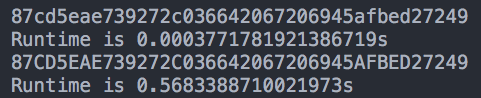
\includegraphics[width=9.62cm, height=1.96cm]{sha1.png}
\caption{SHA1算法测试}
\label{img_sha1}
\end{figure}
% subsection 算法测试 (end)
% section sha1算法 (end)
\section{SHA3算法} % (fold)
\subsection{算法原理} % (fold)
SHA3采用海绵结构,在对明文进行填充后进行分组,再对每一个分组尾部进行填充。初始化矩阵$S$为全0向量,对每个分组,首先将$S$异或该分组更新$S$,然后将$S$转化为三维矩阵$A$,并对$A$进行几个逻辑步函数,得到的输出再更新$S$。再对每个分组都进行操作后,进入挤水阶段。每次将$S$中固定长度的子串取出,然后对$S$再进行一次步函数。如此往复直到取出的所有子串拼接在一起不小于需要的长度,就截取如此长度的子串输出。

SHA3有几种算法:SHA3—224,SHA3-256,SHA3-384,SHA3-512。这几种算法除了参数略有不同以外,并没有很大差异。
% subsection 算法原理 (end)
\subsection{算法实现} % (fold)
我在真正实现时使用了python的numpy相关方法,用于加速以及使代码简洁清晰。这里只给出逻辑。
\begin{enumerate}
    \item SHA3的几种算法的含义
    \begin{lstlisting}[language={python},
    numbers=left,
    numberstyle=\tiny\monaco,
    basicstyle=\small\monaco]
    def SHA3_224(M):
        return bits_to_hex(Keccak(448, M || [0, 1], 224))

    def SHA3_256(M):
        return bits_to_hex(Keccak(512, M || [0, 1], 256))

    def SHA3_384(M):
        return bits_to_hex(Keccak(768, M || [0, 1], 384))

    def SHA3_512(M):
        return bits_to_hex(Keccak(1024, M || [0, 1], 512))

    def Keccak(c, N, d):
        return sponge(1600 - c, N, d)
    \end{lstlisting}
    \item 海绵函数
    \begin{lstlisting}[language={python},
    numbers=left,
    numberstyle=\tiny\monaco,
    basicstyle=\small\monaco]
    def pad(x, m):
        j = (- m - 2) % x
        return [1] || [0] * j || [1]

    def sponge(r, N, d):
        P = N || pad(r, len(N))
        n = len(P) // r
        c = b - r
        part = []
        for i in range(n):
            part.append(P[i*r:(i+1)*r])
        S = [0] * b
        zeroc = [0] * c
        for i in range(n):
            S = Keccak_p(S ^ (part[i] || zeroc))
        Z = []
        while True:
            Z = Z || S[:r]
            if d <= len(Z):
                return Z[:d]
            S = Keccak_p(S)
    \end{lstlisting}
    \item 每一步的操作
    \begin{lstlisting}[language={python},
    numbers=left,
    numberstyle=\tiny\monaco,
    basicstyle=\small\monaco]
    def Keccak_p(S):
        A = string_to_state(S)
        for ir in range(12 + 2 * l - nr, 12 + 2 * l):
            A = Rnd(A, ir)
        return state_to_string(A)

    def Rnd(A, ir):
        return iota(chi(pi(rho(theta(A)))), ir)

    def theta(A):
        C = A[:, 0, :] ^ A[:, 1, :] ^ A[:, 2, :] ^ A[:, 3, :] ^ A[:, 4, :]
        D = (C`x方向循环右移1`) ^ (C`x方向循环左移1,z方向循环右移1`)
        return A[x, y, z] ^= D[x, z]

    def rho(A):
        A1 = 5 * 5 * w `全0矩阵`
        A1[0][0] = A[0][0].copy()
        x, y = 1, 0
        for t in range(24):
            A1[x][y] = A[x][y]  >>> ((t+1)*(t+2)//2)
            x, y = y, (2 * x + 3 * y) % 5
        return A1

    def pi(A):
        A1 = 5 * 5 * w `全0矩阵`
        for x in range(5):
            for y in range(5):
                A1[x][y] = A[(x+3*y) mod 5][x].copy()
        return A1

    def chi(A):
        return A ^ ((A`x方向循环左移1` ^ (5 * 5 * w `全1矩阵`)) & (A`x方向循环左移1`)

    def rc(t):
        if t mod 255 == 0:
            return 1
        r = [1, 0, 0, 0, 0, 0, 0, 0]
        for i in range(t mod 255):
            r = [0] + r
            r[0] ^= r[8]
            r[4] ^= r[8]
            r[5] ^= r[8]
            r[6] ^= r[8]
            r = r[:8]
        return r[0]

    def iota(A, ir):
        A1 = A.copy()
        RC = [0] * w
        for j in range(l + 1):
            RC[(1 << j)-1] = rc(j + 7 * ir)
        A1[0][0] ^= RC
        return A1
    \end{lstlisting}
\end{enumerate}
% subsection 算法实现 (end)
\subsection{算法测试} % (fold)
或许是我的数据结构选取不当,我的SHA3算法速度极慢,只有2~3KB每秒的速度。尽管如此,通过与hashlib的检验,我的算法是正确的。我这里对一个75KB的文件进行SHA3的四种算法的测试,我只在程序里验证了SHA3-224的正确性(其余的正确性已经通过标准样例验证),如图\ref{img_sha3}所示。
\begin{figure}[htbp]
\centering
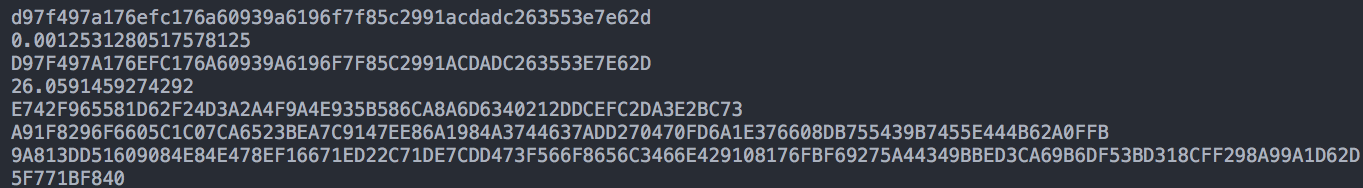
\includegraphics[width=13.63cm, height=1.88cm]{sha3.png}
\caption{SHA3测试}
\label{img_sha3}
\end{figure}
% subsection 算法测试 (end)
% section sha3算法 (end)
\section{HMAC} % (fold)
\subsection{算法原理} % (fold)
HMAC的算法原理就是把密钥和Hash函数结合起来,实现消息认证的目的。其总体逻辑可以概括为以下表达式:
$$MAC(text) = HMAC(K, text) = H((K_0 \oplus opad )|| H((K_0 \oplus ipad) || text))$$
% subsection 算法原理 (end)
\subsection{算法实现} % (fold)
\begin{lstlisting}[language={python},
    numbers=left,
    numberstyle=\tiny\monaco,
    basicstyle=\small\monaco]
    def mac(text):
        ipad = b'\x36' * B
        opad = b'\x5c' * B
        if len(key) > B:
            key = hashFunc(key)
        if len(key) < B:
            key = key.ljust(B, b'\x00')
        ip = ipad ^ key
        hipad = hashFunc(b''.join([ip, text]))
        op = opad ^ key
        return hashFunc(b''.join([op, hipad]))
    \end{lstlisting}
% subsection 算法实现 (end)
\subsection{算法测试} % (fold)
我验证了基于SHA1和SHA3-512的HMAC,并将我的HMAC和python的hmac库内置函数进行比较,结果相同。如图\ref{img_hmac},十六进制大写是我的结果,十六进制小写是内置库的结果,结果一致。
\begin{figure}[htbp]
\centering
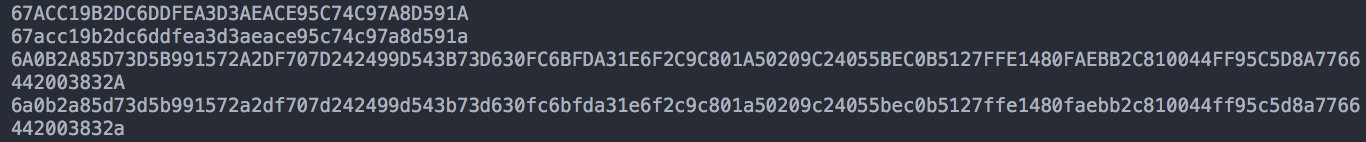
\includegraphics[width=13.66cm, height=1.42cm]{hmac.png}
\caption{HMAC测试}
\label{img_hmac}
\end{figure}
% subsection 算法测试 (end)
% section hmac (end)
\section{简单生日攻击} % (fold)
\subsection{生日攻击原理} % (fold)
生日攻击是一种利用生日悖论攻击Hash函数的攻击。将真消息与假消息同时进行若干同义变换并输入进Hash函数,利用生日悖论有大概率可以找到其中的一对真假消息变形拥有同样的Hash值,从而达到伪造消息也能通过Hash验证的目的。本算法只实现用随机数的方式完成寻找Hash碰撞。
% subsection 生日攻击原理 (end)
\subsection{算法实现} % (fold)
算法利用python的字典实现。将Hash值作为字典的Key,被Hash的消息作为Key对应的Value。每当得到新的消息-Hash对,就以新的Hash值为Key去访问字典,如果发生空Key的错误,就说明没有发生碰撞,则把这一对也加入字典并继续;否则说明有碰撞,直接返回碰撞值。利用try-catch-else的方法可以很好地实现上述算法。
\begin{lstlisting}[language={python},
    numbers=left,
    numberstyle=\tiny\monaco,
    basicstyle=\small\monaco]
    def attack(length):
        birth = {}
        for i in range(1 << 40):
            n = randint(0, 1 << L)
            h = hashFunc(n).hexdigest()[:length]
            try:
                birth[h]
            except KeyError as e:
                birth[h] = n
            else:
                return self.birth[h], n, i
\end{lstlisting}
% subsection 算法实现 (end)
\subsection{算法测试} % (fold)
实际上,想寻找一对完全的Hash碰撞并不容易。这里只能截取Hash输出的前几位进行测试,并调用系统函数库,才能在有生之年看到结果。这里选择的测试结果也只能在十几秒内找到一对前20bit相同的Hash结果。如图\ref{img_attack},这里给出了SHA1算法发生局部碰撞的字节串和其Hash结果。
\begin{figure}[htbp]
\centering
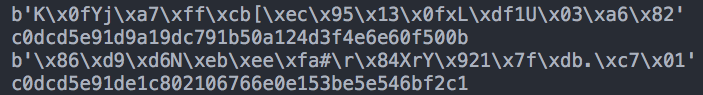
\includegraphics[width=14.06cm, height=1.90cm]{attack.png}
\caption{简单生日攻击测试}
\label{img_attack}
\end{figure}
% subsection 算法测试 (end)
% section 简单生日攻击 (end)
\section{感想} % (fold)
说实话,这种和系统内置库对比的实验任务,真的会一下子让那种“终于把算法调对”的喜悦消失殆尽。或许这种简单实现的算法在效率上就是比不上使用底层库的内置函数——甚至可以说是天壤之别。系统函数在千分之一秒内完成的任务我的算法需要用十几秒才能完成确实让人有挫败感。尽管如此,通过实验透彻理解算法确实让我受益匪浅。功不唐捐。
% section 感想 (end)
\end{document}